\begin{figure}[!t]
\centering
\resizebox{\linewidth}{!}{%
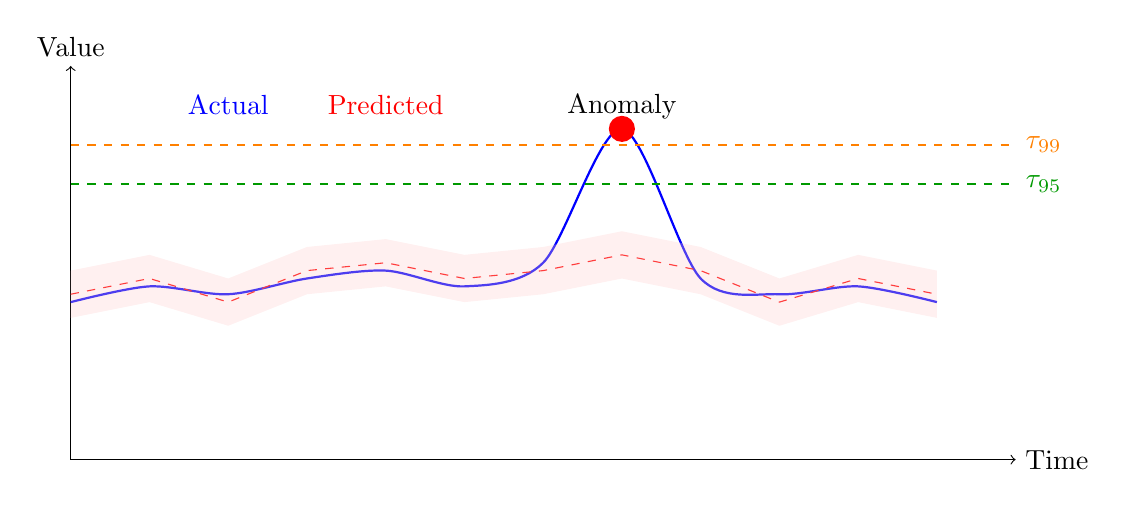
\begin{tikzpicture}
    % Axes
    \draw[->] (0,0) -- (12,0) node[right] {Time};
    \draw[->] (0,0) -- (0,5) node[above] {Value};
    
    % Normal data
    \draw[blue, thick, smooth] plot coordinates {
        (0,2) (1,2.2) (2,2.1) (3,2.3) (4,2.4) (5,2.2) 
        (6,2.5) (7,4.2) (8,2.3) (9,2.1) (10,2.2) (11,2.0)
    };
    
    % Predicted with uncertainty
    \draw[red, dashed] plot coordinates {
        (0,2.1) (1,2.3) (2,2.0) (3,2.4) (4,2.5) (5,2.3) 
        (6,2.4) (7,2.6) (8,2.4) (9,2.0) (10,2.3) (11,2.1)
    };
    
    % Uncertainty bands
    \fill[red!20, opacity=0.3] plot coordinates {
        (0,1.8) (1,2.0) (2,1.7) (3,2.1) (4,2.2) (5,2.0) 
        (6,2.1) (7,2.3) (8,2.1) (9,1.7) (10,2.0) (11,1.8)
    } -- plot coordinates {
        (11,2.4) (10,2.6) (9,2.3) (8,2.7) (7,2.9) (6,2.7) 
        (5,2.6) (4,2.8) (3,2.7) (2,2.3) (1,2.6) (0,2.4)
    } -- cycle;
    
    % Threshold lines
    \draw[green!60!black, thick, dashed] (0,3.5) -- (12,3.5) node[right] {$\tau_{95}$};
    \draw[orange, thick, dashed] (0,4.0) -- (12,4.0) node[right] {$\tau_{99}$};
    
    % Anomaly point
    \node[circle, fill=red, minimum size=0.3cm] at (7,4.2) {};
    \node[above] at (7,4.2) {Anomaly};
    
    % Legend
    \node[blue] at (2,4.5) {Actual};
    \node[red] at (4,4.5) {Predicted};
\end{tikzpicture}%
}
\caption{Anomaly Detection with Uncertainty Bands and Thresholds}
\label{fig:threshold_percentile}
\end{figure}